% !TEX program = xelatex
% ============================================================
% 哈尔滨理工大学 电子信息硕士学位论文 LaTeX 模版
% 编译方式：XeLaTeX → biber → XeLaTeX → XeLaTeX
% 更换内容：正文在 chapters/，前置在 frontmatter/，后置在 backmatter/，
%           图片在 figures/，参考文献在 paper.bib。详见 README.md。
% ============================================================

% ===== 一、字体 =====
\documentclass[UTF8, 12pt]{ctexart}

% 英文字体
\usepackage{fontspec}
\setmainfont{Times New Roman}

% 中文字体说明：
%   正文用宋体（SimSun）、标题用黑体（SimHei）。这两个是 Windows 系统字体，
%   有版权、未随仓库分发；请自行将 simsun-win.ttc、SimHei.ttf 放入 ./fonts/ 目录
%   （获取方式见 fonts/README.md）。仿宋、楷体使用 TeX Live 自带的开源 Fandol，无需另装。
%   若暂时没有宋体/黑体文件，可注释掉下面这段、改用本节末尾的「Fandol 兜底方案」。
\setCJKmainfont[
  Path = ./fonts/,
  UprightFont = simsun-win.ttc,
  AutoFakeBold = 2.5
]{SimSun}                                  % 宋体 → 正文
\setCJKsansfont[
  Path = ./fonts/,
  UprightFont = SimHei.ttf
]{SimHei}                                  % 黑体 → 标题
\setCJKmonofont{FandolFang}                % 仿宋 → 等宽位

\setCJKfamilyfont{zhsong}[
  Path = ./fonts/,
  UprightFont = simsun-win.ttc,
  AutoFakeBold = 2.5
]{SimSun}
\setCJKfamilyfont{zhhei}[
  Path = ./fonts/,
  UprightFont = SimHei.ttf
]{SimHei}
\setCJKfamilyfont{zhkai}{FandolKai}
\setCJKfamilyfont{zhfs}{FandolFang}

% ---------- Fandol 兜底方案（开箱即用，无需宋体/黑体文件）----------
% 没有 Windows 宋体/黑体时，注释掉上面整段中文字体设置，改用下面这段：
% （TeX Live / Overleaf 自带 Fandol，可直接编译，仅与宋体/黑体观感略有差异）
%
% \setCJKmainfont{FandolSong}
% \setCJKsansfont{FandolHei}
% \setCJKmonofont{FandolFang}
% \setCJKfamilyfont{zhsong}{FandolSong}
% \setCJKfamilyfont{zhhei}{FandolHei}
% \setCJKfamilyfont{zhkai}{FandolKai}
% \setCJKfamilyfont{zhfs}{FandolFang}
% ------------------------------------------------------------------

% ===== 二、页面设置 =====
\usepackage{geometry}
\geometry{
  a4paper,
  top=4.4cm,
  bottom=4.3cm,
  left=3.25cm,
  right=3.25cm,
  headheight=15pt,
  headsep=0.521cm,
  footskip=0.95cm,
}

% ===== 三、常用宏包 =====
\usepackage{amsmath,amssymb}
\usepackage{graphicx}
\usepackage{float}
\usepackage{array}
\usepackage{longtable}
\usepackage{booktabs}
\usepackage{titlesec}
\usepackage{titletoc}
\usepackage{CJKfntef}
\usepackage{caption}
\usepackage{chngcntr}
\usepackage{fancyhdr}
\usepackage{etoolbox}
\usepackage{placeins}


% ===== 四、章节计数器（article 模拟章节编号）=====
\newcounter{chapternum}
\newcommand{\setchapternum}[1]{%
  \setcounter{chapternum}{#1}%
  \setcounter{equation}{0}%
  \setcounter{figure}{0}%
  \setcounter{table}{0}%
}
\renewcommand{\theequation}{\arabic{chapternum}-\arabic{equation}}
\counterwithin{figure}{chapternum}
\counterwithin{table}{chapternum}
\renewcommand{\thefigure}{\arabic{chapternum}-\arabic{figure}}
\renewcommand{\thetable}{\arabic{chapternum}-\arabic{table}}
\providecommand*{\theHequation}{\arabic{chapternum}.\arabic{equation}}
\providecommand*{\theHfigure}{\arabic{chapternum}.\arabic{figure}}
\providecommand*{\theHtable}{\arabic{chapternum}.\arabic{table}}

% ===== 五、参考文献 & 超链接 =====
\usepackage[
  backend=biber,
  style=gb7714-2015,
  autocite=inline,
  sorting=none,
  gbnamefmt=lowercase,
  sortcites=true,
  gbcitelabel=bracket,
  gbcitecomp=true,
  maxbibnames=3,      % 超过3人显示 et al.
  minbibnames=3,      % et al. 前保留3个作者
  gbtype=true,
  gbpunctin=false,
  gbfieldstd=true
]{biblatex}
\AtBeginBibliography{\renewrobustcmd*{\mkbibemph}[1]{#1}}
% 取消斜体
\addbibresource{paper.bib}

\usepackage{hyperref}
\hypersetup{
  hidelinks,
  pdfborder={0 0 0},
  hypertexnames=false
}

% 为了和word的标题段前段后空隙保持一致
\newcommand{\xiaoer}{\fontsize{18pt}{25.2pt}\selectfont}   % 18 × 1.4
\newcommand{\xiaosan}{\fontsize{15pt}{21pt}\selectfont}    % 15 × 1.4
\newcommand{\sihao}{\fontsize{14pt}{19.6pt}\selectfont}    % 14 × 1.4

% ===== 六、字号命令 =====
% \newcommand{\xiaoer}{\fontsize{18pt}{21.6pt}\selectfont}
% \newcommand{\xiaosan}{\fontsize{15pt}{18pt}\selectfont}
% \newcommand{\sihao}{\fontsize{14pt}{16.8pt}\selectfont}
\newcommand{\xiaosi}{\fontsize{12pt}{18pt}\selectfont}
\newcommand{\xiaowu}{\fontsize{9pt}{10.8pt}\selectfont}
\newcommand{\wuhao}{\fontsize{10.5pt}{12.6pt}\selectfont}

% ===== 七、正文默认字号与段落 =====
\AtBeginDocument{\linespread{1}\xiaosi\setlength{\parindent}{2em}\setlength{\parskip}{0pt}\setlength{\emergencystretch}{1em}}

% ===== 八、章节标题格式 =====
% 一级标题：黑体小二，居中，段前12pt 段后6pt，单倍行距
\titleformat{\section}[block]
  {\centering\heiti\xiaoer\linespread{1}\selectfont}
  {第\thesection 章}{1em}{\strut}
\titlespacing{\section}{0pt}{12pt}{12pt}

\titleformat{\subsection}[block]
  {\heiti\xiaosan\linespread{1}\selectfont}
  {\thesubsection}{1em}{\strut}
\titlespacing{\subsection}{0pt}{6pt}{6pt}

\titleformat{\subsubsection}[block]
  {\heiti\sihao\linespread{1}\selectfont}
  {\thesubsubsection}{1em}{\strut}
\titlespacing{\subsubsection}{0pt}{3pt}{3pt}

% 四级（runin）
\titleformat{\paragraph}[runin]
  {\heiti\xiaosi\linespread{1}\selectfont}
  {}{0pt}{}
\titlespacing{\paragraph}{2em}{6pt}{1em}

% ===== 十、图表标题 =====
\DeclareCaptionFont{wuhao}{\wuhao}
\captionsetup{font={wuhao,stretch=1},justification=centering,singlelinecheck=false,labelsep=space}
\captionsetup[figure]{position=bottom,skip=6pt}
\captionsetup[table]{position=top,skip=6pt}
\AtBeginEnvironment{tabular}{\wuhao}
\AtBeginEnvironment{tabular*}{\wuhao}
\AtBeginEnvironment{longtable}{\wuhao}
\setlength{\heavyrulewidth}{1.5pt}
\setlength{\lightrulewidth}{1pt}
\setlength{\cmidrulewidth}{1pt}

% ===== 十一、目录 =====

% 配置章目录格式 (第1级)
\titlecontents{section}[0pt] % 左缩进
  {\heiti\zihao{-4}} % 字体格式：黑体，小4号
  {第\thecontentslabel 章\quad} % 章节号格式：第x章 + 标题
  {} % 节标题
  {\tocdotfill\tocpage} % 填充点线及页码

% 配置节目录格式 (第2级)
\titlecontents{subsection}[3em] % 缩进：约3.5个汉字宽
  {\songti\zihao{-4}} % 字体格式：宋体，小4号
  {\contentslabel{1.5em}} % 节号盒宽：约2.8个汉字宽
  {}
  {\tocdotfill\tocpage} % 填充点线及页码

\titlecontents{subsubsection}[4.5em] % 缩进：再右移一档
  {\songti\zihao{-4}} % 字体格式：宋体，小4号
  {\contentslabel{2em}} % 节号盒宽：约4.0个汉字宽
  {}
  {\tocdotfill\tocpage} % 填充点线及页码

\renewcommand{\contentsname}{\centering 目 \quad 录}
\newcommand{\tocdotfill}{\titlerule*[0.30pc]{{\normalfont.}}}
\newcommand{\tocpage}{\normalfont\contentspage}

% ===================================================================
\begin{document}

% 去掉页眉罗马数字编码
\pagenumbering{Roman}
\fancypagestyle{plain}{
  \fancyhf{}
  \fancyfoot[C]{\wuhao -\Roman{page}-}
  \renewcommand{\headrulewidth}{0pt}   % 不显示线
}
\pagestyle{plain}

% 中英文摘要
% 中文标题（过长可用 \\ 手动换行）
\section*{基于卷积神经网络的手写数字识别方法研究}

\section*{摘 \quad 要}
\addcontentsline{toc}{section}{摘要}


手写数字识别是模式识别与图像分类领域的经典问题，应用广泛。传统方法依赖人工设计的特征，泛化能力有限，而卷积神经网络能够自动学习层次化特征，更适合此类任务。本文以 MNIST 数据集为对象，设计一种小型卷积神经网络：以四个 $3\times3$ 卷积层配合批量归一化与 ReLU，经两次最大池化后由全连接层完成分类，参数量约 0.47M。


在此基础上，本文研究了数据增强、批量归一化、Dropout 与 Adam 优化等训练方法的作用。实验表明，所提方法在 MNIST 测试集上取得 99.32\% 的识别准确率，优于 Softmax 回归、多层感知机与 LeNet-5 等对比方法，消融实验也验证了各训练技巧的有效性。


\vspace{\baselineskip}

% 关键词（用分号分隔）
{\noindent
\begingroup
\setbox0=\hbox{\textbf{关键词}\quad}
\hangindent=\wd0
\hangafter=1
\textbf{关键词}\quad 卷积神经网络；手写数字识别；MNIST；深度学习；图像分类\par
\endgroup
}

\clearpage
\section*{\textbf{Research on Handwritten Digit Recognition Based on Convolutional Neural Networks}}


\section*{\textbf{Abstract}}
\addcontentsline{toc}{section}{Abstract}


Handwritten digit recognition is a classic problem in pattern recognition and image classification with wide applications. Traditional methods rely on hand-crafted features and exhibit limited generalization, whereas convolutional neural networks can automatically learn hierarchical features and are better suited to this task. Taking the MNIST dataset as the research object, this thesis designs a lightweight convolutional neural network: four $3\times3$ convolutional layers with batch normalization and ReLU, followed by two max-pooling operations and fully connected layers for classification, with about 0.47M parameters in total.


On this basis, the thesis investigates the roles of data augmentation, batch normalization, Dropout, and the Adam optimizer. Experiments show that the proposed method achieves a recognition accuracy of 99.32\% on the MNIST test set, outperforming Softmax regression, the multilayer perceptron, and LeNet-5, while the ablation study verifies the effectiveness of each training technique.


\vspace{\baselineskip}

{\noindent
\begingroup
\raggedright
\setbox0=\hbox{\textbf{Keywords}\quad}
\hangindent=\wd0
\hangafter=1
\makebox[\wd0][l]{\textbf{Keywords}\quad}convolutional~neural~network, handwritten~digit~recognition, MNIST, deep~learning, image~classification\par
\endgroup
}

\clearpage

% 补回页眉
\pagestyle{fancy}
\fancyhead[C]{\songti\xiaowu 哈尔滨理工大学电子信息硕士学位论文}
\renewcommand{\headrulewidth}{0.4pt}
\newcommand{\wordthickthinrule}{%
  \par\noindent
  \hrule height 1.0bp
  \vskip 0.5bp
  \hrule height 0.5bp
  \par
}
\makeatletter
\renewcommand{\headrule}{\wordthickthinrule}
\makeatother
\fancyfoot[C]{\wuhao -\thepage-}

% 目录
\tableofcontents
\clearpage

% 正文同时开始阿拉伯数字编码
\pagenumbering{arabic}
\addtocontents{toc}{\vspace{1em}}   % ← 摘要与绪论之间空一行
% 每章第一行用 \section{} 作为「第 X 章」标题；第二行 \setchapternum{X} 设定本章号，
% 图、表、公式会自动按「X-序号」编号。正文用 \cite 命令引用 paper.bib 中的文献。
\section{绪论}
\setchapternum{1}

\subsection{研究背景与意义}

手写数字识别是模式识别与计算机视觉领域的经典问题，在邮政编码分拣、票据处理、表单录入等场景中应用广泛。传统方法依赖人工设计的特征与分类器，泛化能力有限；近年来卷积神经网络凭借自动特征学习的能力在图像分类任务中取得突破\cite{lecun2015deep}，为手写数字识别提供了更为有效的途径。

\subsection{国内外研究现状}

卷积神经网络自 LeNet\cite{lecun1998gradient} 提出以来不断演进，AlexNet\cite{krizhevsky2012imagenet}、VGG\cite{simonyan2015very}、GoogLeNet\cite{szegedy2015going}、ResNet\cite{he2016deep} 等模型相继将图像分类精度推向新高，批量归一化\cite{ioffe2015batch}、Dropout\cite{srivastava2014dropout} 等技术也显著提升了网络的可训练性与泛化能力。在手写数字识别方面，MNIST\cite{deng2012mnist} 已成为最常用的标准基准，国内亦有大量相关研究与综述\cite{zhou2017cnn,li2016cnn}。

\subsection{研究内容与论文结构}

本文以 MNIST 数据集为对象，设计一种小型卷积神经网络，并研究数据增强、批量归一化、Dropout 等训练优化方法对识别性能的影响，最终在测试集上取得 99.32\% 的识别准确率。全文共分五章：第一章为绪论；第二章介绍相关理论与技术基础；第三章给出网络结构设计；第四章讨论模型训练与优化；第五章为实验与结果分析；最后为结论。

\clearpage
\section{相关理论与技术基础}
\setchapternum{2}

本章简要介绍本文方法所依托的理论基础，包括人工神经网络与卷积神经网络的基本组成，以及实验所用的 MNIST 数据集。

\subsection{人工神经网络基础}

人工神经网络由大量神经元分层连接而成。单个神经元对输入 $x_1,\dots,x_n$ 加权求和并经激活函数 $f(\cdot)$ 输出，如式(\ref{eq:neuron})所示。网络参数通过反向传播算法\cite{rumelhart1986learning}与梯度下降进行训练。

% ===== 带编号公式示例（编号自动为「2-序号」）=====
\begin{equation}
a = f\!\left( \sum_{i=1}^{n} w_i x_i + b \right)
\label{eq:neuron}
\end{equation}

\subsection{卷积神经网络}

卷积神经网络针对图像数据引入局部连接、权值共享与下采样机制，能够自动学习由低级到高级的层次化特征，相比全连接网络大幅减少了参数量\cite{lecun1998gradient,goodfellow2016deep}。其典型结构由卷积层、池化层交替堆叠，最后接全连接层完成分类，如图\ref{fig:cnn-arch}所示。

% ===== 插图示例（图片放在 figures/ 目录；中英文图题用 \\ 换行）=====
\begin{figure}[htb]
\centering
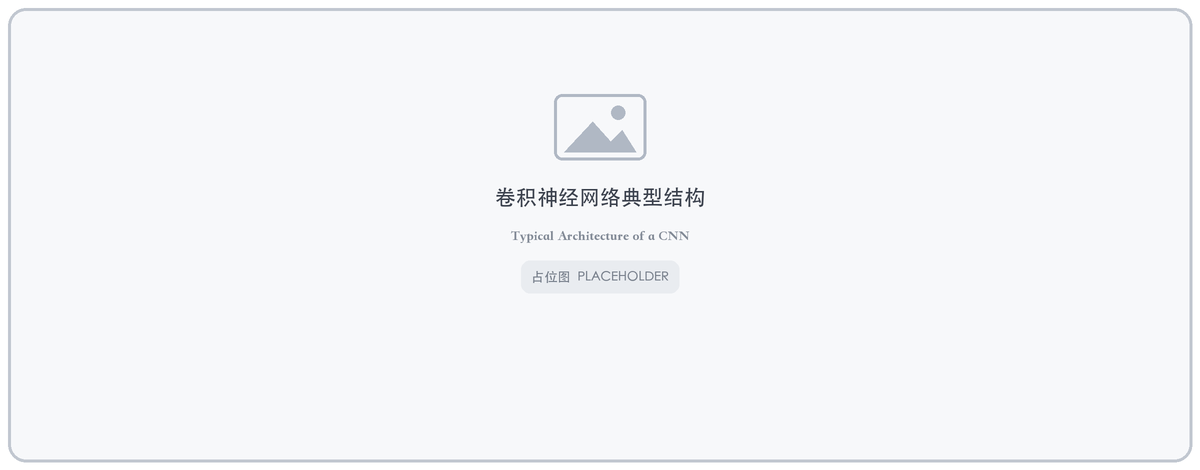
\includegraphics[width=0.95\linewidth]{figures/fig-cnn-architecture.png}
\caption{卷积神经网络典型结构\\Fig.~\thefigure\ Typical architecture of a convolutional neural network}
\label{fig:cnn-arch}
\end{figure}

\subsubsection{卷积层}

卷积层通过卷积核在输入特征图上滑动提取局部特征。设输入宽度为 $W$、卷积核大小为 $K$、填充为 $P$、步长为 $S$，则输出特征图宽度如式(\ref{eq:convsize})所示，高度同理。本文采用 $3\times3$ 卷积核并通过权值共享降低参数量。

\begin{equation}
W' = \frac{W - K + 2P}{S} + 1
\label{eq:convsize}
\end{equation}

\subsubsection{激活函数与池化}

为引入非线性，本文在卷积层后采用修正线性单元（ReLU）\cite{nair2010rectified}，其定义为 $f(x)=\max(0,x)$，可有效缓解梯度消失并加速收敛。池化层用于下采样，本文采用 $2\times2$ 最大池化，在保留显著特征的同时将特征图尺寸减半，并增强对微小位移的鲁棒性。

\subsection{MNIST 数据集}

MNIST 是手写数字识别领域应用最广的标准基准\cite{lecun1998gradient,deng2012mnist}，包含 $60{,}000$ 张训练图像与 $10{,}000$ 张测试图像，每张为 $28\times28$ 灰度图，对应 $0\sim9$ 共十个类别。

\subsection{本章小结}

本章梳理了人工神经网络与卷积神经网络的基本原理，并介绍了实验数据集，为后续网络设计与实验奠定基础。

\clearpage
\section{基于卷积神经网络的手写数字识别网络设计}
\setchapternum{3}

\subsection{设计原则}

针对 MNIST 图像尺寸小、为单通道灰度图的特点，本文以「参数量小、易于训练、精度高」为设计目标，借鉴堆叠 $3\times3$ 小卷积核加深网络的思想\cite{simonyan2015very}，并引入批量归一化\cite{ioffe2015batch}、ReLU 激活\cite{nair2010rectified}与 Dropout\cite{srivastava2014dropout}以稳定训练、抑制过拟合。

\subsection{网络结构}

本文设计的网络如图\ref{fig:network}所示：输入经四个 $3\times3$ 卷积层（通道数 $32,32,64,64$，均配批量归一化与 ReLU）与两次 $2\times2$ 最大池化逐步提取特征，再由两个全连接层（$3136\rightarrow128\rightarrow10$）完成分类，逐层配置见表\ref{tab:layers}。

\begin{figure}[htb]
\centering
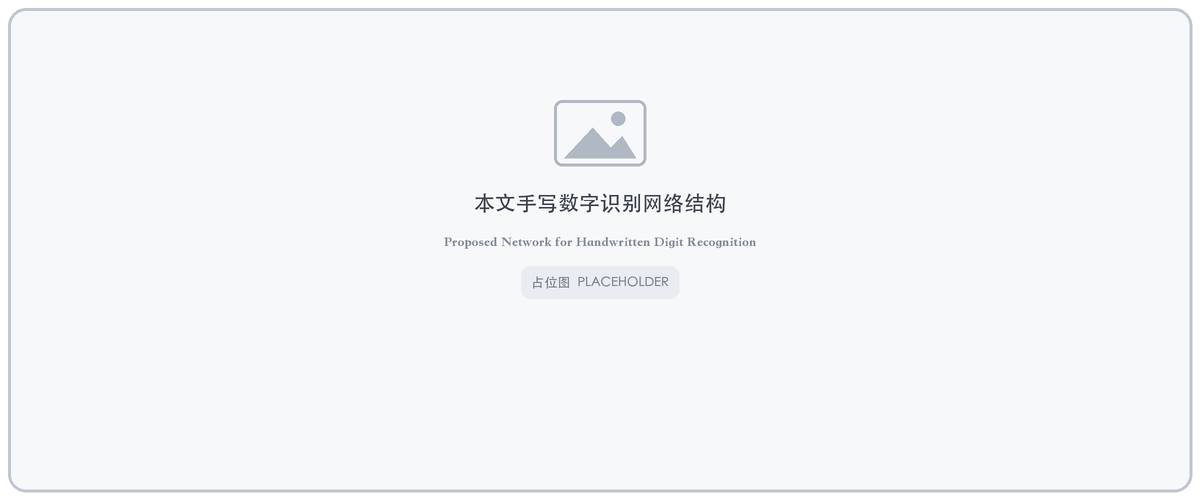
\includegraphics[width=0.95\linewidth]{figures/fig-network-design.png}
\caption{本文手写数字识别网络结构\\Fig.~\thefigure\ Architecture of the proposed network}
\label{fig:network}
\end{figure}

% ===== 三线表示例（booktabs：\toprule / \midrule / \bottomrule；\label 紧跟 \caption）=====
\begin{table}[htbp]
\centering
\caption{本文网络逐层结构配置\\Table~\thetable\ Layer-wise configuration of the proposed network}
\label{tab:layers}
\begin{tabular*}{\linewidth}{@{\extracolsep{\fill}}c c c c}
\toprule
层名称 & 类型 & 输出尺寸 & 卷积核/参数 \\
\midrule
输入 & --- & $1\times28\times28$ & --- \\
Conv1 & 卷积+BN+ReLU & $32\times28\times28$ & $3\times3,\ 32,\ \text{pad}=1$ \\
Conv2 & 卷积+BN+ReLU & $32\times28\times28$ & $3\times3,\ 32,\ \text{pad}=1$ \\
Pool1 & 最大池化 & $32\times14\times14$ & $2\times2$ \\
Conv3 & 卷积+BN+ReLU & $64\times14\times14$ & $3\times3,\ 64,\ \text{pad}=1$ \\
Conv4 & 卷积+BN+ReLU & $64\times14\times14$ & $3\times3,\ 64,\ \text{pad}=1$ \\
Pool2 & 最大池化 & $64\times7\times7$ & $2\times2$ \\
FC1 & 全连接+ReLU+Dropout & $128$ & $3136\times128$ \\
FC2 & 全连接 & $10$ & $128\times10$ \\
输出 & Softmax & $10$ & --- \\
\bottomrule
\end{tabular*}
\end{table}

卷积层参数量由式(\ref{eq:param})估算，据此可得全网参数量约为 $0.47\text{M}$，其中全连接层占绝大部分，卷积层因权值共享而参数很少，整体结构轻量、易于训练。

\begin{equation}
N_{\text{conv}} = K\times K\times C_{\text{in}}\times C_{\text{out}} + C_{\text{out}}
\label{eq:param}
\end{equation}

\subsection{本章小结}

本章给出了本文小型卷积神经网络的设计原则与逐层结构，参数量约 $0.47\text{M}$，为下一章的训练与优化奠定基础。

\clearpage
\section{模型训练与优化}
\setchapternum{4}

\subsection{数据预处理与增强}

训练前先将像素归一化至 $[0,1]$ 并按训练集统计量标准化。为提升泛化能力，训练阶段在线施加随机旋转（$\pm10^{\circ}$）、随机平移（$\pm2$ 像素）与随机缩放等数据增强\cite{krizhevsky2012imagenet}，测试阶段不作增强。

\subsection{损失函数与优化器}

本文采用交叉熵损失，如式(\ref{eq:ce})所示，其中 $N$ 为样本数、$C=10$ 为类别数、$p_{i,c}$ 为预测概率。优化器选用 Adam\cite{kingma2015adam}，初始学习率 $0.001$，批大小 $128$。

\begin{equation}
\mathcal{L} = -\frac{1}{N}\sum_{i=1}^{N}\sum_{c=1}^{C} \mathbb{1}\{y_i = c\}\log p_{i,c}
\label{eq:ce}
\end{equation}

\subsection{正则化方法}

% ===== 四级标题（runin 嵌入式）示例 =====
\paragraph{批量归一化。}通过对每层输入按小批量归一化\cite{ioffe2015batch}，缓解内部协变量偏移，加速收敛并稳定训练。

\paragraph{Dropout。}在全连接层以 $0.5$ 的概率随机失活神经元\cite{srivastava2014dropout}，近似集成多个子网络，有效抑制过拟合；卷积层与全连接层权重采用 He 初始化\cite{glorot2010understanding}。

\subsection{训练设置与消融实验}

实验基于 PyTorch 实现，在单张 NVIDIA RTX 3060 GPU 上训练 $20$ 轮。为评估各训练技巧的贡献，本文以基础 CNN 为对照逐项叠加，结果如表\ref{tab:ablation}所示：三项技巧累计使测试准确率从 $98.74\%$ 提升至 $99.32\%$。

\begin{table}[htbp]
\centering
\caption{训练技巧消融实验结果\\Table~\thetable\ Ablation study of training techniques}
\label{tab:ablation}
\begin{tabular*}{\linewidth}{@{\extracolsep{\fill}}c c c}
\toprule
配置 & 测试准确率 (\%) & 相对提升 \\
\midrule
基础 CNN & 98.74 & --- \\
\quad + 批量归一化 & 99.05 & +0.31 \\
\quad + Dropout & 99.18 & +0.13 \\
\quad + 数据增强（本文方法） & 99.32 & +0.14 \\
\bottomrule
\end{tabular*}
\end{table}

\subsection{本章小结}

本章介绍了数据增强、交叉熵损失与 Adam 优化器，以及批量归一化、Dropout 等正则化方法，并通过消融实验验证了各项训练技巧的有效性。

\clearpage
\section{实验与结果分析}
\setchapternum{5}

\subsection{实验环境与设置}

实验基于 Python 与 PyTorch 框架，在单张 NVIDIA RTX 3060 GPU 上完成。严格遵循 MNIST 标准划分，在 $60{,}000$ 张训练样本上训练、在独立的 $10{,}000$ 张测试样本上评估，训练配置与第四章一致。

\subsection{评价指标}

本文采用准确率（式(\ref{eq:acc})）作为主要指标，并辅以精确率、召回率及其调和平均 F1 分数（式(\ref{eq:f1})）。对十个类别取宏平均以反映整体性能。

\begin{equation}
\mathrm{Accuracy} = \frac{TP + TN}{TP + TN + FP + FN}
\label{eq:acc}
\end{equation}

\begin{equation}
\mathrm{F1} = \frac{2 \times \mathrm{Precision} \times \mathrm{Recall}}{\mathrm{Precision} + \mathrm{Recall}}
\label{eq:f1}
\end{equation}

\subsection{结果与对比分析}

各方法在 MNIST 测试集上的准确率如表\ref{tab:comparison}所示。本文方法达到 $99.32\%$，显著优于线性的 Softmax 回归与全连接的多层感知机，并较经典的 LeNet-5\cite{lecun1998gradient}进一步提升，体现了卷积结构与训练优化策略的有效性\cite{goodfellow2016deep}。

\begin{table}[htbp]
\centering
\caption{不同方法在 MNIST 测试集上的准确率对比\\Table~\thetable\ Accuracy comparison of different methods on MNIST}
\label{tab:comparison}
\begin{tabular*}{\linewidth}{@{\extracolsep{\fill}}c c c}
\toprule
方法 & 测试准确率 (\%) & 备注 \\
\midrule
Softmax 回归 & 92.0 & 线性分类器 \\
多层感知机（MLP） & 98.1 & 全连接网络 \\
LeNet-5 & 98.9 & 经典卷积网络 \\
\textbf{本文方法} & \textbf{99.32} & 本文 CNN \\
\bottomrule
\end{tabular*}
\end{table}

\subsection{训练过程与错误分析}

训练损失与测试准确率随轮次的变化如图\ref{fig:curve}所示，模型在约第 $10\sim15$ 轮趋于收敛，训练与测试表现差距较小，无明显过拟合。测试集混淆矩阵如图\ref{fig:confusion}所示，绝大多数样本集中于对角线，错误主要发生在书写形近的数字对（如 $4$ 与 $9$、$3$ 与 $5$）之间。

\begin{figure}[htb]
\centering
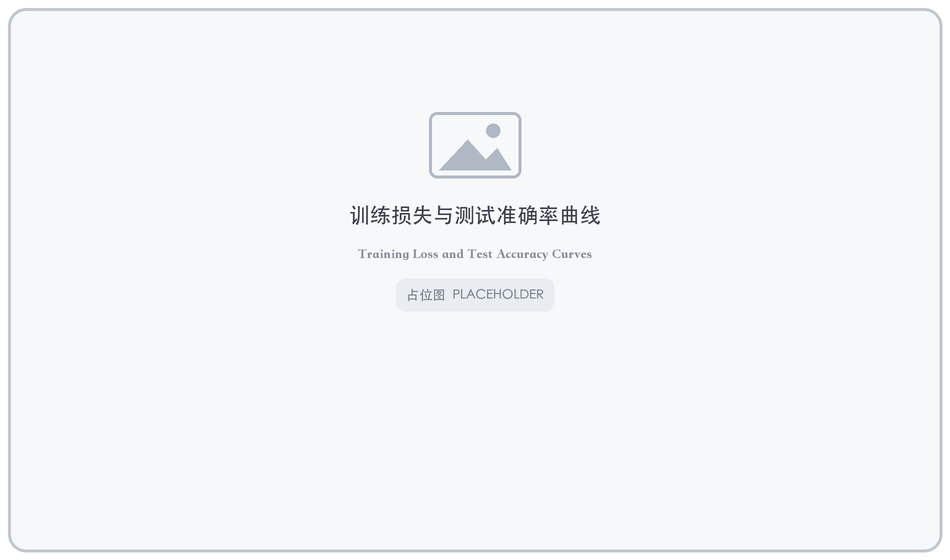
\includegraphics[width=0.85\linewidth]{figures/fig-training-curve.png}
\caption{训练损失与测试准确率曲线\\Fig.~\thefigure\ Training loss and test accuracy curves}
\label{fig:curve}
\end{figure}

\begin{figure}[htb]
\centering
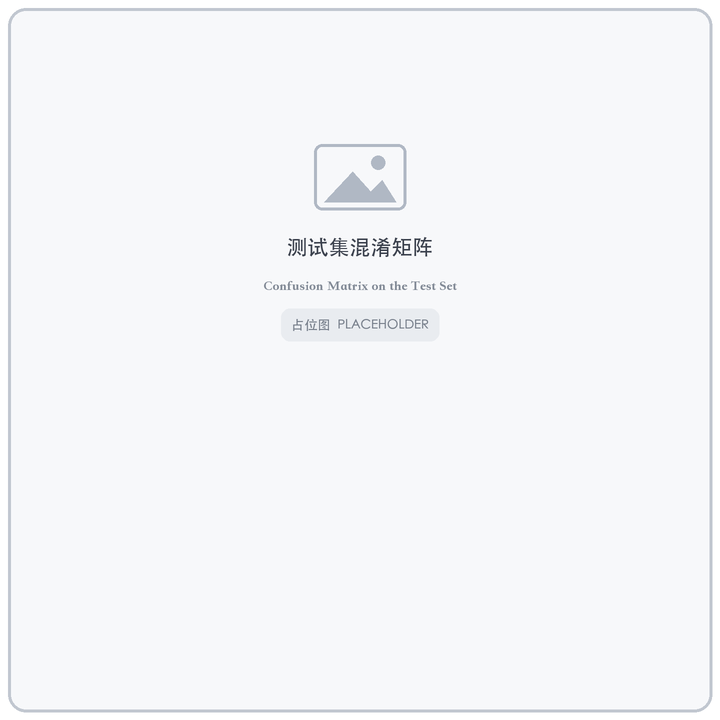
\includegraphics[width=0.7\linewidth]{figures/fig-confusion-matrix.png}
\caption{测试集混淆矩阵\\Fig.~\thefigure\ Confusion matrix on the test set}
\label{fig:confusion}
\end{figure}

\subsection{本章小结}

本章在 MNIST 数据集上验证了本文方法，测试准确率达 $99.32\%$，优于各对比方法，且收敛稳定、泛化良好。

\clearpage

\phantomsection
\section*{结 \quad 论}
\addcontentsline{toc}{section}{结论}


本文面向 MNIST 手写数字识别任务，设计了一种参数量约 0.47M 的小型卷积神经网络，并系统研究了数据增强、批量归一化、Dropout 与自适应优化等训练方法。实验表明，所提方法在测试集上取得 99.32\% 的识别准确率，优于 Softmax 回归、多层感知机与 LeNet-5 等对比方法，消融实验验证了各训练技巧的独立贡献。


本文方法仍存在不足：实验仅在 MNIST 这一相对规整的数据集上验证，对更复杂的真实手写场景，其泛化能力有待进一步检验；网络结构与训练策略也有优化空间。未来可在更具挑战性的数据集上开展实验，并探索残差连接、注意力机制以及模型压缩等方向。

\clearpage
\begingroup
\sloppy
\phantomsection
\printbibliography[heading=bibintoc,title={参考文献}]
\endgroup
\clearpage
% 本页为示例占位内容，请替换为本人攻读学位期间的真实成果（论文/专利/软著/竞赛等）。
\phantomsection
\section*{攻读硕士学位期间发表的学术论文及获得成果}
\addcontentsline{toc}{section}{攻读硕士学位期间发表的学术论文及获得成果}

\begingroup
\setlength{\parskip}{0pt}
\setcounter{enumi}{0}
\newlength{\resultlabelwidth}
\newcommand{\resultitem}{%
  \par\addvspace{\bibitemsep}%
  \stepcounter{enumi}%
  \settowidth{\resultlabelwidth}{\mkgbnumlabel{\arabic{enumi}}}%
  \setlength{\hangindent}{\dimexpr\resultlabelwidth+\biblabelsep\relax}%
  \noindent\mkgbnumlabel{\arabic{enumi}}\hspace{\biblabelsep}%
}
  \resultitem 张三, 李四. 基于卷积神经网络的手写数字识别方法研究[J]. 示例学报, 2025, 42(3): 100--108.（示例，请替换）
  \resultitem 实用新型专利：一种示例装置，某某大学。\newline
        申请号：ZL2025XXXXXXXXX.X，申请时间：2025 年 X 月 X 日。
  \resultitem 软件著作权：示例软件系统 V1.0，某某大学。\newline
        登记号：2025SRXXXXXXX，授权时间：2025 年 X 月 X 日。
  \resultitem 竞赛获奖：张三，某某大学，某某竞赛省级一等奖，2025 年 X 月。
\par
\endgroup

\clearpage
% 本页为示例占位内容，请替换为本人的真实致谢（下文“XXX”处请填写实际姓名）。
\phantomsection
\section*{致 \quad 谢}
\addcontentsline{toc}{section}{致谢}


值此论文完成之际，谨向所有给予我帮助和支持的人致以诚挚的谢意。首先感谢我的导师 XXX 老师，从论文选题、研究方案到论文撰写，导师始终给予悉心指导，其严谨的治学态度与认真负责的精神令我受益匪浅。


同时，感谢研究生期间各位授课老师的教导，感谢实验室同学与朋友的帮助和陪伴，也感谢家人一直以来的支持与鼓励，使我能够顺利完成学业。


\end{document}
